\documentclass{report}

% Language setting
% Replace `english' with e.g. `spanish' to change the document language
\usepackage[english]{babel}

% Set page size and margins
% Replace `letterpaper' with `a4paper' for UK/EU standard size
\usepackage[letterpaper,top=2cm,bottom=2cm,left=3cm,right=3cm,marginparwidth=1.75cm]{geometry}

% Useful packages
\usepackage{amsmath}
\usepackage{graphicx}
\usepackage[colorlinks=true, allcolors=blue]{hyperref}
\usepackage[style=ieee, backend=biber]{biblatex}
\addbibresource{bibliography.bib}
\usepackage{csquotes}

\title{High Performance Computing Project - A.A. 2022/2023}
\author{Andres Bermeo Marinelli}

\begin{document}
\maketitle
\tableofcontents
\chapter{Benchmarking MKL, OpenBLAS, and BLIS}

\section{Introduction}

In this exercise we compare the performance of three High Performance Libraries
(HPC): MKL, OpenBLAS, and BLIS. In particular, we focus on the level 3 BLAS 
function called \texttt{gemm}, which multiples an $m \times k$ matrix $A$ times 
a $k \times n$ matrix $B$ and stores the result in an $m \times n$ matrix $C$. 

This function comes in two types, one for single 
precision (float) and the other for double precision (double). Furthermore, it 
is capable of exploiting paralellism using OpenMP (OMP) to speed up the 
calculations, provided that we have the required computational resources.

Using squared matrices only, we perform a scalability study in two scenarios. 
In the first scenario, we fix the number of cores, and increase the size of the
matrices from $2000$ to $20000$. In the second scenario, we fix the matrix size 
to $10000$ and increase the number of cores that \texttt{gemm} can use by 
modifying the \texttt{OMP\_NUM\_THREADS} environment variable.

In both scenarios, we repeat the measurements for both single and double
precision, for both THIN and EPYC nodes, using the maximum number of cores.

Furthermore, for the second scenario, we also modify the thread affinity policy 
of OMP in order to observe any differences.

\section{Methodology}

\subsection{Compiling BLIS and obtaining binaries}

We begin by downloading the BLIS library by using the following commands:
\begin{verbatim}
    $git clone https://github.com/flame/blis.git
    $cd blis
    $srun -p {NODE} -n1 ./configure --enable-cblas --enable-threading=openmp --prefix=/path/to/myblis/lib auto
    $srun -p {NODE} -n 1 --cpus-per-task={P} make -j {P}
    $make install
\end{verbatim}

Where \texttt{NODE} can be specified as either \texttt{THIN} or \texttt{EPYC} and 
\texttt{P} are the available cores for each node, $24$ and $128$ respectively.

With these commands, we have compiled the BLIS library for the desired 
architecture.

Next, we specify the flag in the Makefile to compile for float or double using 
\texttt{\-DUSE\_FLOAT} or \texttt{\-DUSE\_DOUBLE}. Then, we run:
\begin{verbatim}
    $salloc -n {P} -N1 -p {NODE} --time=1:0:0
    $module load mkl/latest
    $module load openBLAS/0.3.23-omp
    $export LD_LIBRARY_PATH=/path/to/myblis/lib:$LD_LIBRARY_PATH
    $srun -n1 make cpu
\end{verbatim}

Which will generate the binaries for the desired architecture, with floar or 
double precision, depending on the flag we used.

To run, we use: 
\begin{verbatim}
    $srun -n1 --cpus-per-task=128  ./gemm_mkl.x {size_M} {size_K} {size_N}
    $srun -n1 --cpus-per-task=128  ./gemm_oblas.x {size_M} {size_K} {size_N}
    $srun -n1 --cpus-per-task=128  ./gemm_blis.x {size_M} {size_K} {size_N}
\end{verbatim}

At the end of this procedure, we should have the appropriate binaries for each 
architecture, and for each type of precision, double or float.

We now detail the steps to obtain the measurements for both scenarios.

\subsection{Using a fixed number of cores}

For this section, we use all the cores available in a THIN or an EPYC node: 24 
and 128, respectively. 

Since we only use squared matrices, we can describe the dimensions of the matrices 
with a single number, which we call "size". 

For both architectures, we start with a size of $2000$ and end with a size of 
$20000$, with jumps of $2000$ for a total of $10$ sizes. For each size, 
we repeat the measurement $10$ times and report the average and standard 
deviation.

Finally, we repeat the measurements for both floating point precision and double 
point precision.

The scripts that were used can be found in the folder \texttt{exercise2/scripts}, 
under the name \texttt{es2\_1\_thin.sh} and \texttt{es2\_1\_epyc.sh}.

It is important to observe that in this section, since we are using the entire 
node, there is little possibility to play with combinations of thread affinity.

This will be done for the next section.

Furthermore, contrary to the guidelines for the exercise, we decided to use the 
entire node to benchmark its full capacity, and also to avoid wasting 
resources. 

In fact, to obtain an accurate benchmark, we need to reserve the whole node, 
regardless of the number of cores we decide to use. This is because if other 
people began to use the other half of the node, this could introduce additional 
workloads which interfere with the benchmark. 

\subsection{Using a fixed matrix size}

For this section, we fix the size of the matrices to $10000$. Then, we slowly 
increase the number of cores to be used, until we reach the maximum. 

To set the number of cores, we change the environment variable 
\texttt{OMP\_NUM\_THREADS} to the desired value.

For THIN nodes, which have $24$ cores, we start using $1$ core, then $2$ and 
then we increase by steps of $2$, for a total of 13 points.

For EPYC nodes, which have $128$ cores, we start from $1$, then $10$ and then 
we increase by steps of $10$ until $120$. We also use $128$ cores, to see what 
happens at full capacity. We obtain a total of $14$ points.

We repeat all measurements $10$ times and report the average and standard 
deviation.

As usual, we repeat this process for both floating and double point precision.

In this section, we have the liberty to explore different thread allocation 
policies since we are not always using the whole node. 

We decided to use following combinations:
\begin{enumerate}
    \item \texttt{OMP\_PLACES=cores} and \texttt{OMP\_PROC\_BIND=close} 
    \item \texttt{OMP\_PLACES=cores} and \texttt{OMP\_PROC\_BIND=spread} 
\end{enumerate}

The scripts that were used can be found in the folder \texttt{exercise2/scripts}, 
under the names \texttt{es2\_2\_close\_thin.sh}, \texttt{es2\_2\_close\_epyc.sh}, 
\texttt{es2\_2\_spread\_thin.sh}, and \texttt{es2\_2\_spread\_epyc.sh}.

\section{Results and Discussion}

Before we discuss the results of both exercises individually, we briefly 
introduce the equation to calculate the theoretical peak performance ($T_{pp}$) 
of a machine:

\begin{equation}
    T_{pp} = \text{Core Count}\times \text{clock freq.} \times \text{IPC}
\end{equation}

Where \texttt{IPC} is the instructions per cycle that the architecture 
is capable of executing.

This equation is very intuitive. The clock frequency tells us how many cycles 
per second a single core is able to achieve. The ipc factor tells us how many 
instructions per cycle the core can execute. This number is different for 
single precision (SP) and double precision (DP) operations. Finally, we need 
to multiple this by the number of cores that our machine has. 

On orfeo, THIN and EPYC nodes are composed of: 
\begin{itemize}
    \item THIN: $24$ Intel(R) Xeon(R) Gold $6126$ CPU's at $2.60$GHz - Skylake
    \item EPYC: $128$ EPYC AMD 7H12 CPU's at $2.60$GHz - Zen 2 (7002 a.k.a "Rome")
\end{itemize}

Skylake architecture is reported\cite{arch} to be able to execute $64$ SP FLOP per cycle 
and $32$ DP FLOP per cycle. On the other hand, Zen 2 is reported\cite{arch} to execute 
$32$ SP FLOP per cycle and $16$ DP FLOP per cycle.

Therefore, we obtain: 

\begin{table}[h]
\centering
\begin{tabular}{c|c|c|c|c|c|}
    Node Type & Total Cores & IPC (SP) & IPC (DP) & $T_{pp}$ (SP) & $T_{pp}$ (DP)\\\hline
    THIN      &     24      &    64    &   32     & $\sim 4$ TFLOPS & $\sim 2$ TFLOPS \\
    EPYC      &    128      &    32    &   16     & $\sim 10.6$ TFLOPS & $\sim 5.3$ TFLOPS \\
\end{tabular}
\caption{\label{tab:perf}Performance table of THIN and EPYC node architectures.}
\end{table}

Now we can proceed to discuss the results of the exercise.

\subsection{Using a fixed number of cores}

As mentioned above, in this section, we keep the number of cores fixed to the 
maximum available in the node, and we slowly increase the size of the matrices 
being multiplied from $m=2000$ to $m=20000$. 

\subsubsection{THIN Nodes}

\begin{figure}[h!]
% \centering
\hspace*{-2.5cm}
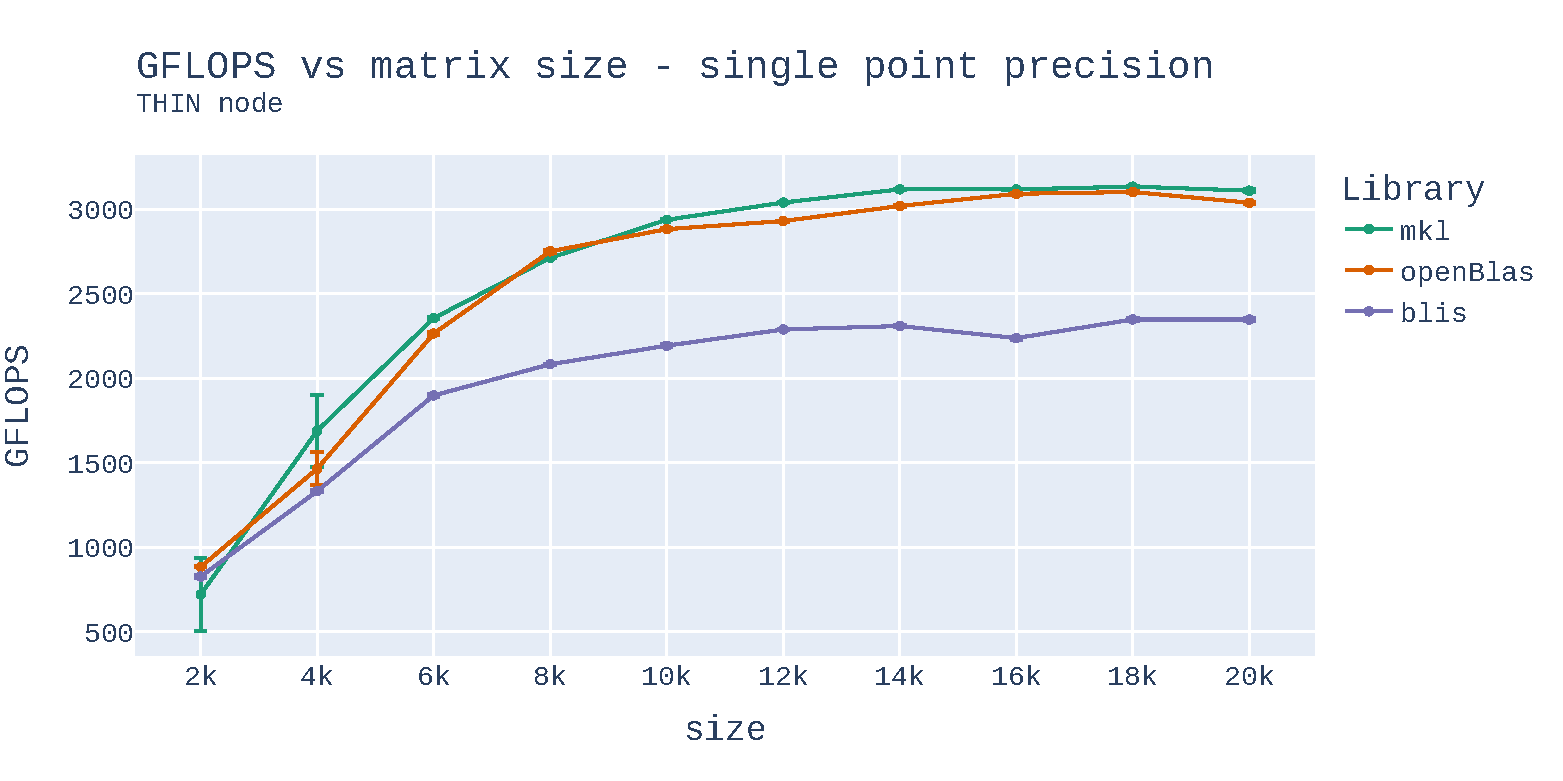
\includegraphics[width=10cm, height=6cm]{./images/fixed_cores_thin_float_gflops.pdf}
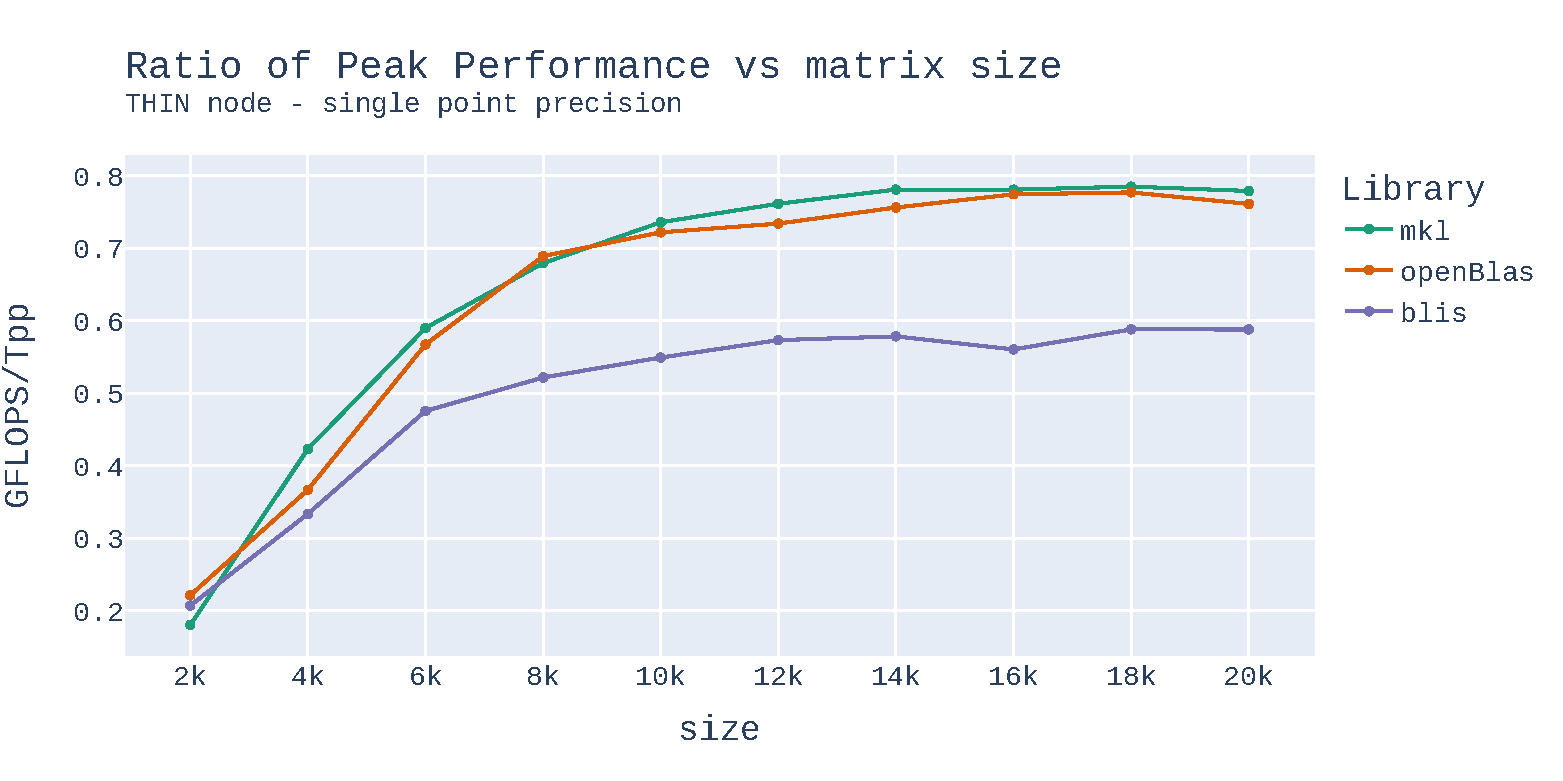
\includegraphics[width=10cm, height=6cm]{./images/fixed_cores_thin_float_gflops_ratio.pdf}
\caption{\label{fig:fixed_cores_thin_float} Results of SP matrix-matrix multiplication 
for THIN nodes. \texttt{MKL} and \texttt{OpenBLAS} perform similarly, outperforming 
\texttt{BLIS} for all matrix sizes.}
\end{figure}
We see that both \texttt{MKL} and 
\texttt{OpenBLAS} are able to reach $\sim 3.2$ TFLOPS, which is around 
$80\%$ of $T_{pp}$. On the other hand, the \texttt{BLIS} library is not 
able to exploit the full potential of the machine, arriving only to 
$\sim 2.4$ TFLOPS, which is $60\%$ of $T_{pp}$.

\begin{figure}[h!]
% \centering
\hspace*{-2.5cm}
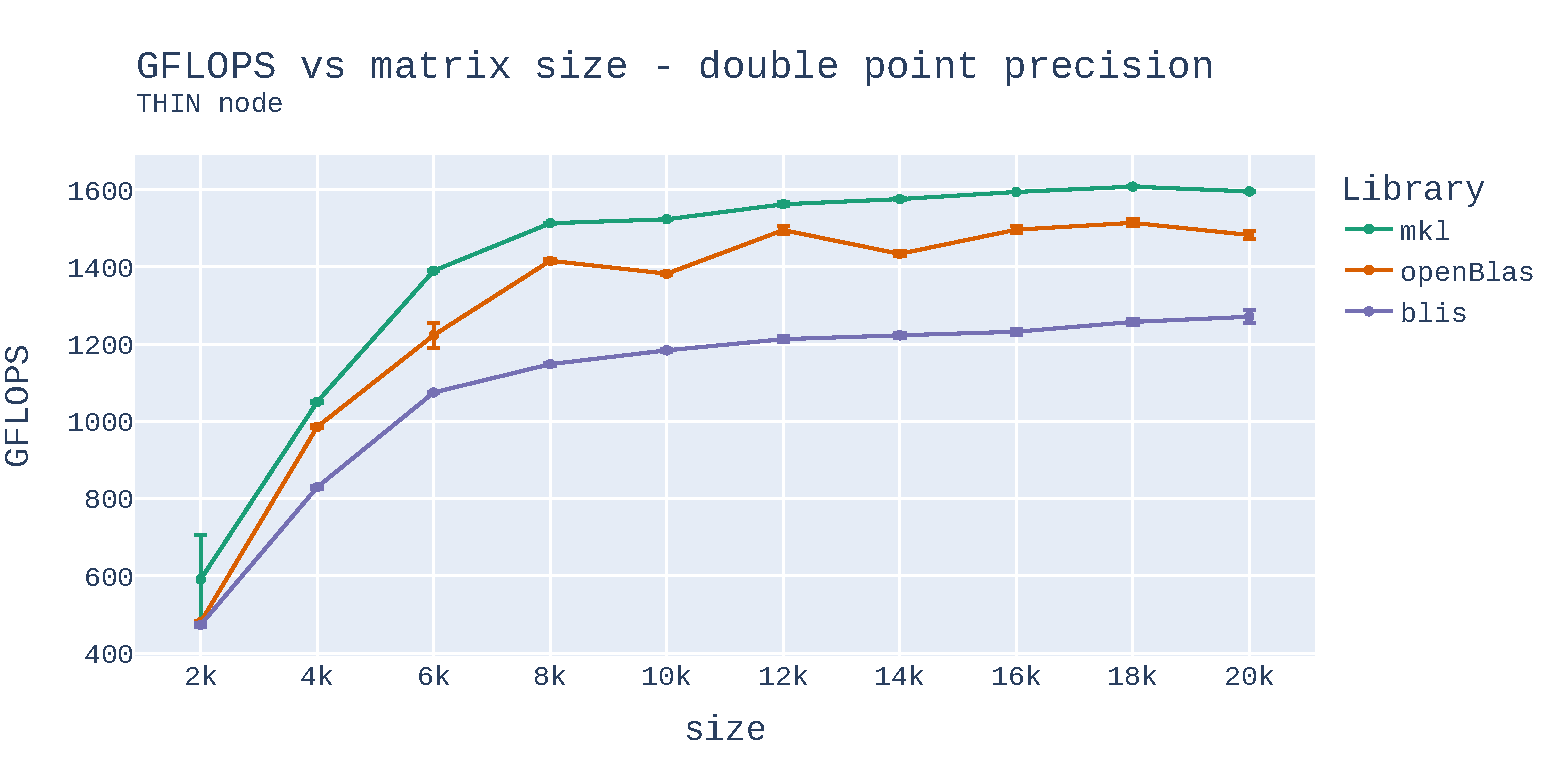
\includegraphics[width=10cm, height=6cm]{./images/fixed_cores_thin_double_gflops.pdf}
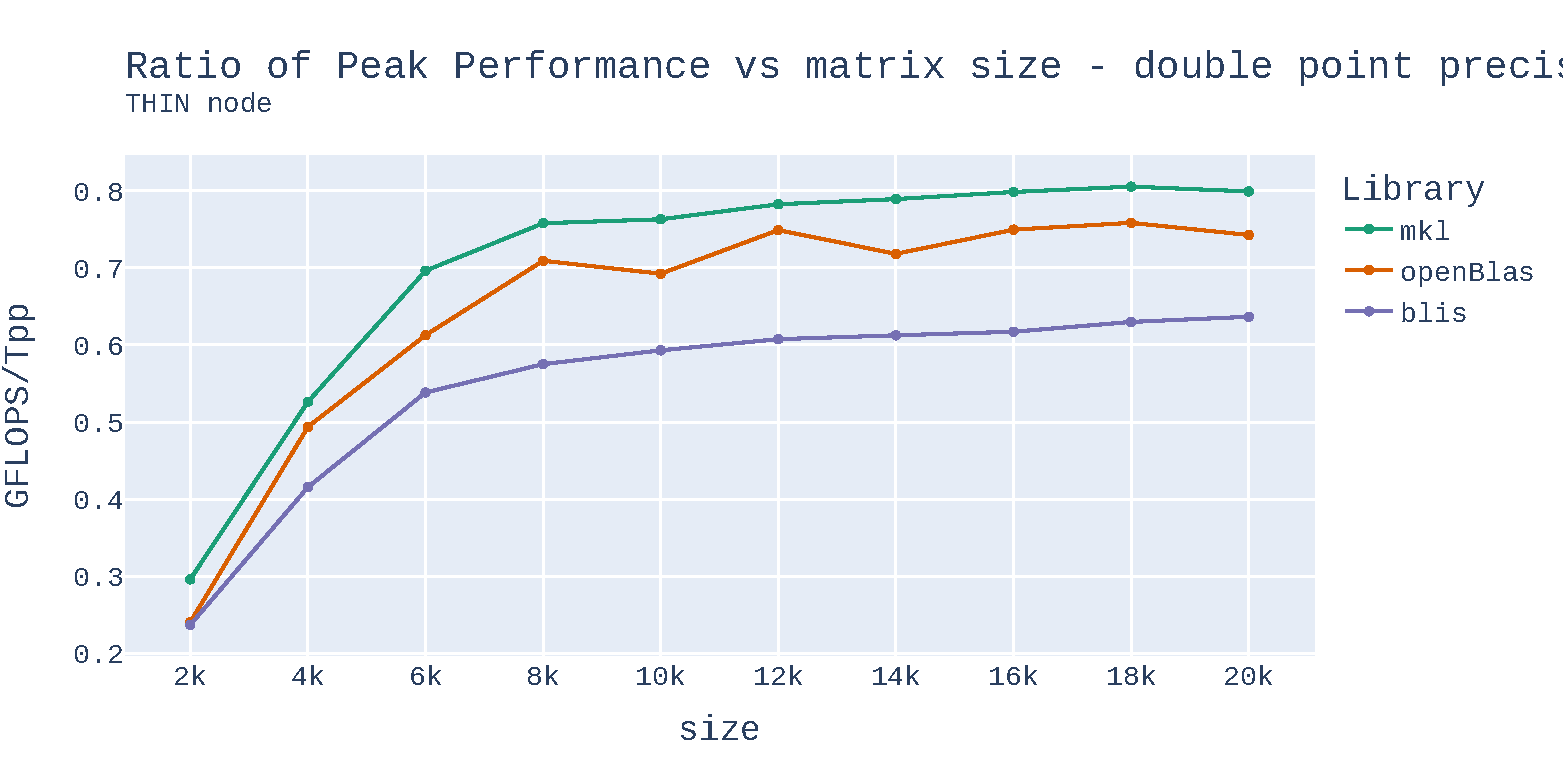
\includegraphics[width=10cm, height=6cm]{./images/fixed_cores_thin_double_gflops_ratio.pdf}
\caption{\label{fig:fixed_cores_thin_double} Results of DP matrix-matrix multiplication 
for THIN nodes. \texttt{MKL} performs the best, slightly above \texttt{OpenBLAS}. 
Both outperform \texttt{BLIS} for all matrix sizes.}
\end{figure}
We see that \texttt{MKL} reaches $\sim1.6$ TFLOPS, 
while \texttt{OpenBLAS} is slightly lower, at $\sim1.5$ TFLOPS, which is $\sim80\%$ and 
$\sim75\%$ of $T_{pp}$, respectively. On the other hand, \texttt{BLIS} arrives to 
$\sim1.3$ TFLOPS, which is $\sim65\%$ of $T_{pp}$.

For both graphs, we notice that on \texttt{MKL} and \texttt{OpenBLAS} are better 
able to exploit the full potential of a THIN node. On the other hand, \texttt{BLIS}
seems to only be able to arrive to $\sim 60\%$ of $T_{pp}$. Therefore, on THIN nodes, 
if we need to multiply two matrices on THIN, we should always use the first 
two libraries to get some more performance. To get the absolute best performance, 
it is preferable to use \texttt{MKL}.

Notice that this statement is true for both single and double precision, and for 
the whole range of matrix sizes we have analyzed. 

These results shouldn't be surprising, considering 
that \texttt{MKL} is developed by Intel, and THIN nodes are Intel based.
Therefore, we expect that this library is very fine tuned to their own architecture 
and is able to exploit the performance of their machines.

Lastly, we observe the impressive results achieved by \texttt{OpenBLAS} which 
is based on the original implementation of Kazushige Goto, and is able to achieve a similar performance to 
\texttt{MKL}, which is maintained by an entire corporation.

\subsubsection{EPYC Nodes}

Now we show the results for the same computations on EPYC nodes, which have a 
$T_{pp}$ of $10.6$ TFLOPS for SP and $5.3$ TFLOPS for DP.

\begin{figure}[h!p]
% \centering
\hspace*{-2.5cm}
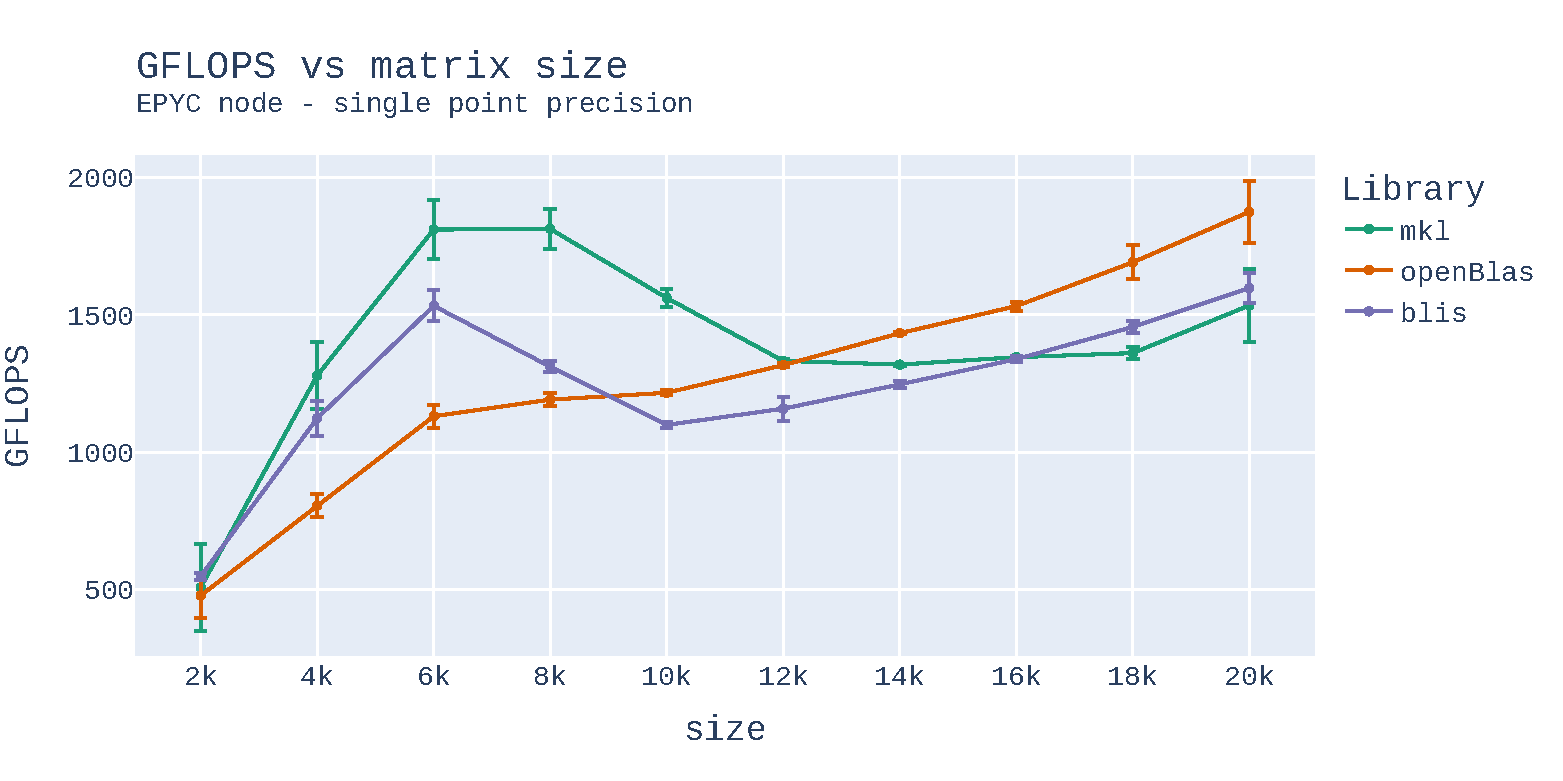
\includegraphics[width=10cm, height=6cm]{./images/fixed_cores_epyc_float_gflops.pdf}
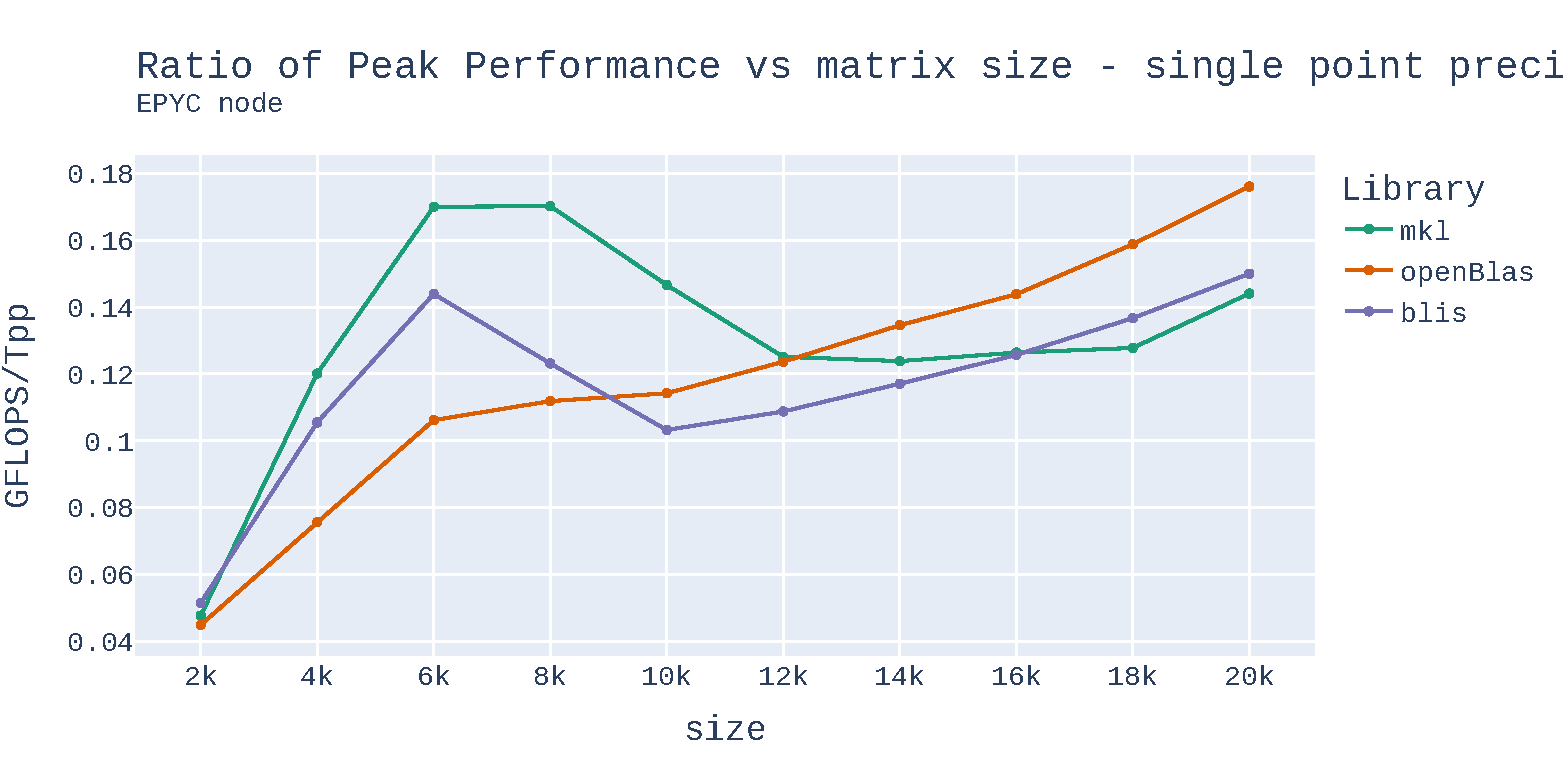
\includegraphics[width=10cm, height=6cm]{./images/fixed_cores_epyc_float_gflops_ratio.pdf}
\caption{\label{fig:fixed_cores_epyc_float} Results of SP matrix-matrix multiplication 
for EPYC nodes. We notice that asymptotically, \texttt{OpenBLAS} outperforms 
\texttt{MKL} and \texttt{BLIS}, while for small matrices, \texttt{OpenBLAS} 
performs the worst.}
\end{figure} 

In this case, we obtain some results. None of the libraries are able to reach 
more than $20\%$ of $T_{pp}$. Furthermore, for matrices of size $\leq 9000$, 
\texttt{MKL} and \texttt{BLIS} outperform \texttt{OpenBLAS}. Between sizes 
$9000$ and $12000$, \texttt{MKL} performs best, and \texttt{OpenBLAS} begins to 
perform better than \texttt{BLIS}. For sizes $\geq 12000$, \texttt{OpenBLAS} 
performs the best.

\begin{figure}[h!p]
% \centering
\hspace*{-2.5cm}
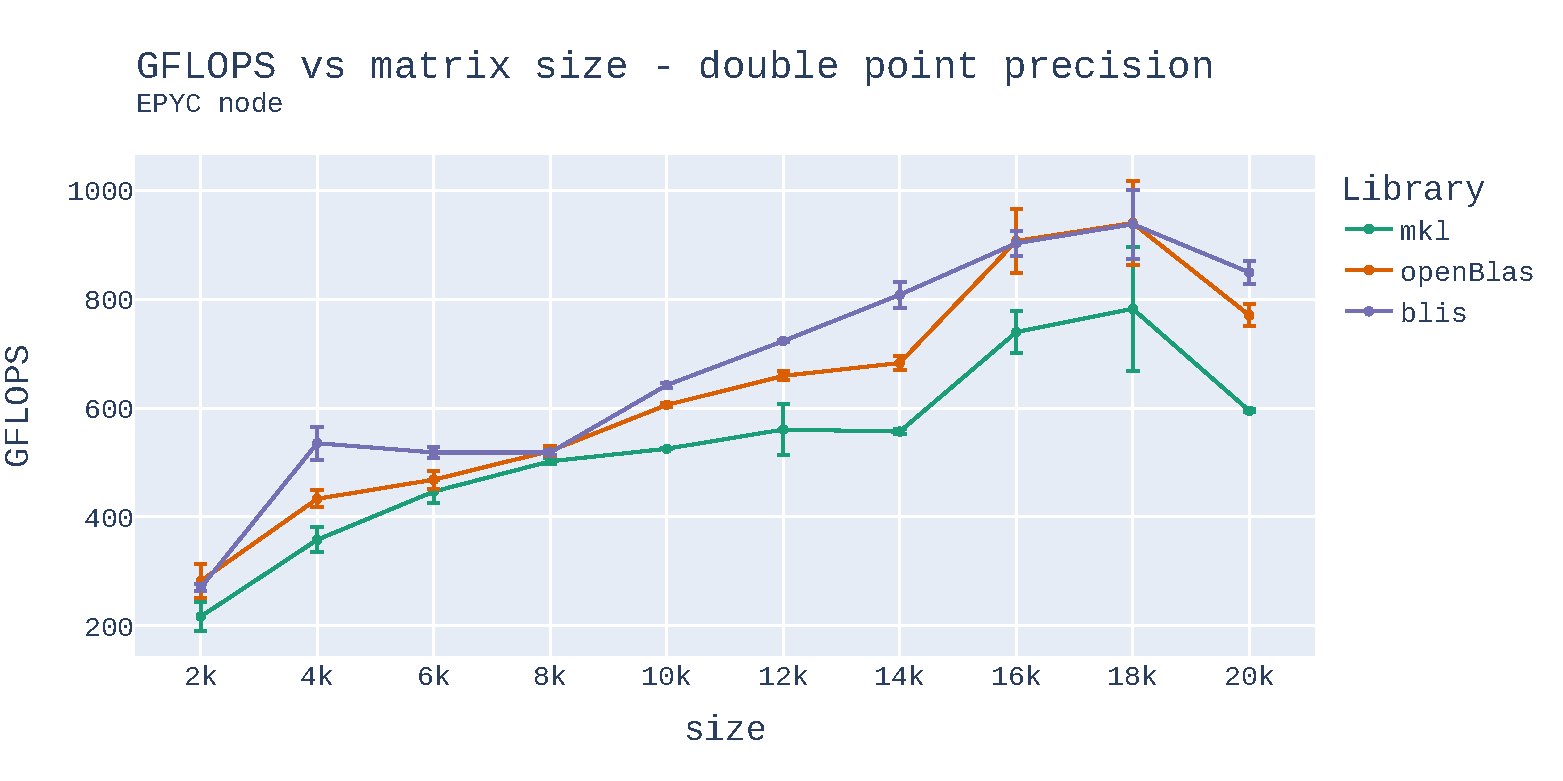
\includegraphics[width=10cm, height=6cm]{./images/fixed_cores_epyc_double_gflops.pdf}
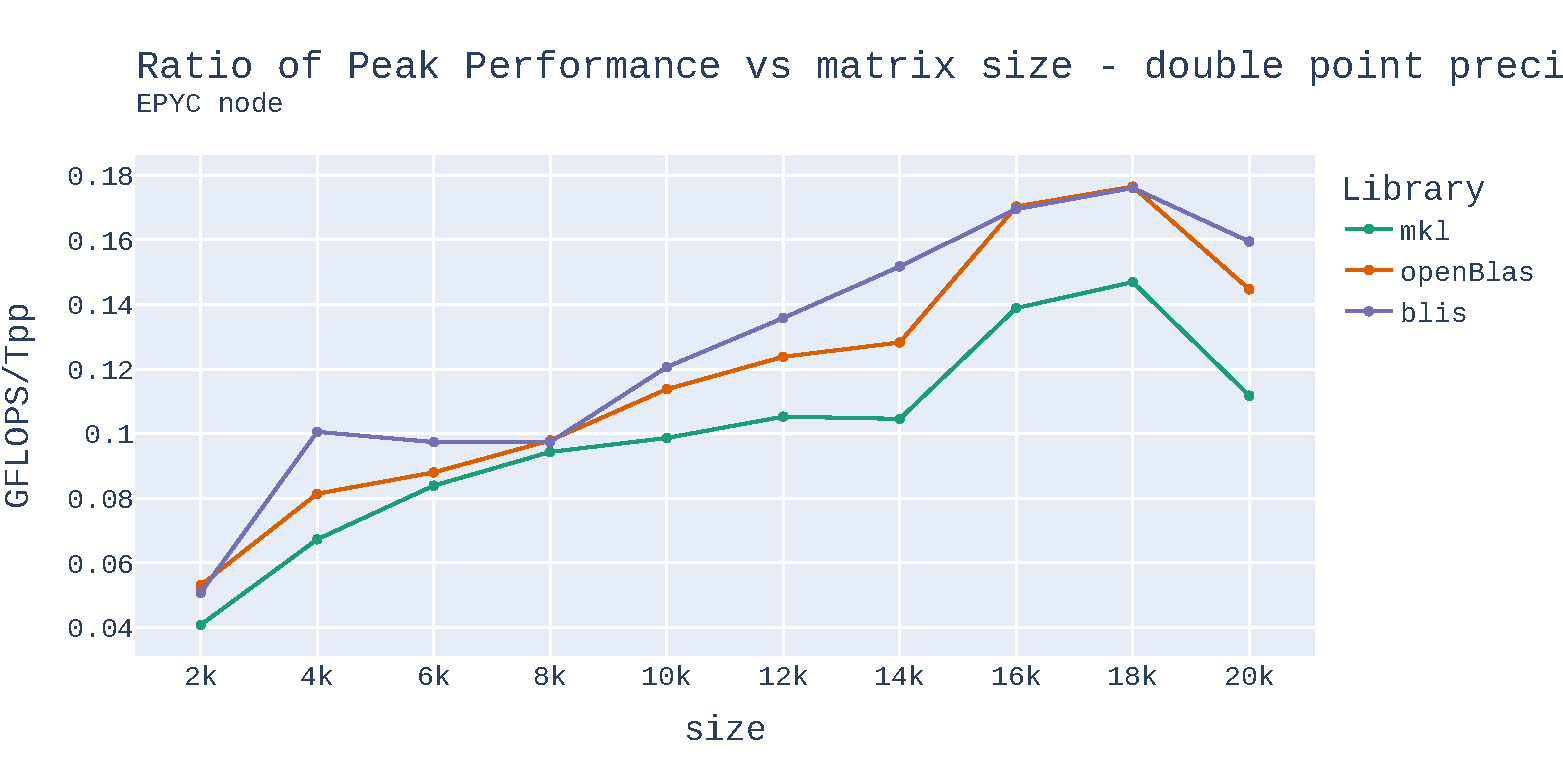
\includegraphics[width=10cm, height=6cm]{./images/fixed_cores_epyc_double_gflops_ratio.pdf}
\caption{\label{fig:fixed_cores_epyc_double} Results of DP matrix-matrix multiplication 
for EPYC nodes. \texttt{BLIS} outperforms \texttt{MKL} and \texttt{OpenBLAS}, 
for all matrix sizes.}

\end{figure}
Again, we notice that none of the libraries are able to achieve more than $20\%$ 
of $T_{pp}$. However, in this case, \texttt{BLIS} outperforms the other two libraries 
for all matrix sizes. The next best performer is \texttt{OpenBLAS}, followed by 
\texttt{MKL}, which performs the worst.

In conclusion, on EPYC nodes, it seems that for DP matrix-matrix multiplication, 
it is better to use \texttt{BLIS}, while for SP, it is very dependant on the 
size of the matrices. However, for large matrices, we should use \texttt{OpenBLAS}
while for smaller ones, we should use \texttt{MKL}. 

\subsection{Using a fixed matrix size}

In this section, we fix the matrix size to $10000$ and we slowly increase the 
amount of cores that the libraries can exploit for multithrading, through OMP. 
For THIN nodes, we arrive to $24$ cores, while for EPYC nodes, we arrive to $128$ 
cores.

Furthermore, since we are slowly increasing the number of cores that the libraries 
can use for multithreading, we can study the effects of using different 
thread allocation policies.

As mentioned above, we chose to always use \texttt{OMP\_PLACES=cores} for these 
experiments. However, we used both \texttt{OMP\_PROC\_BIND=close} and 
\texttt{OMP\_PROC\_BIND=spread}. In the first case, the threads will occupy first 
one entire socket, and then, when it is full, the other socket. In the second case, 
the threads will be placed as spread as possible, on two sockets. 
In both cases, when we use the full node, we expect the results to be the same.

\subsubsection{THIN Nodes}
\begin{figure}[h!]
% \centering
\hspace*{-2.5cm}
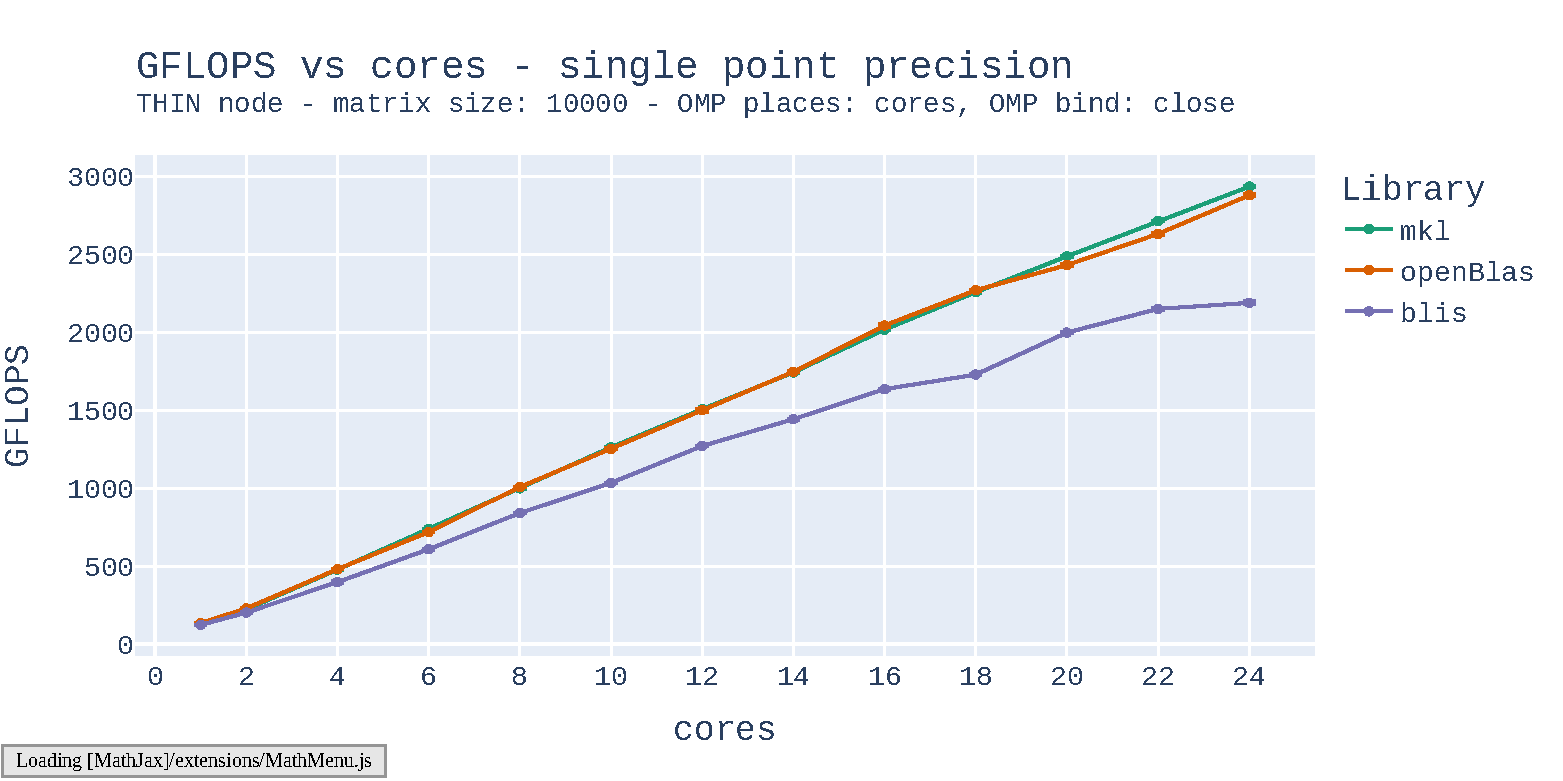
\includegraphics[width=10cm, height=6cm]{./images/fixed_size_thin_float_gflops_close.pdf}
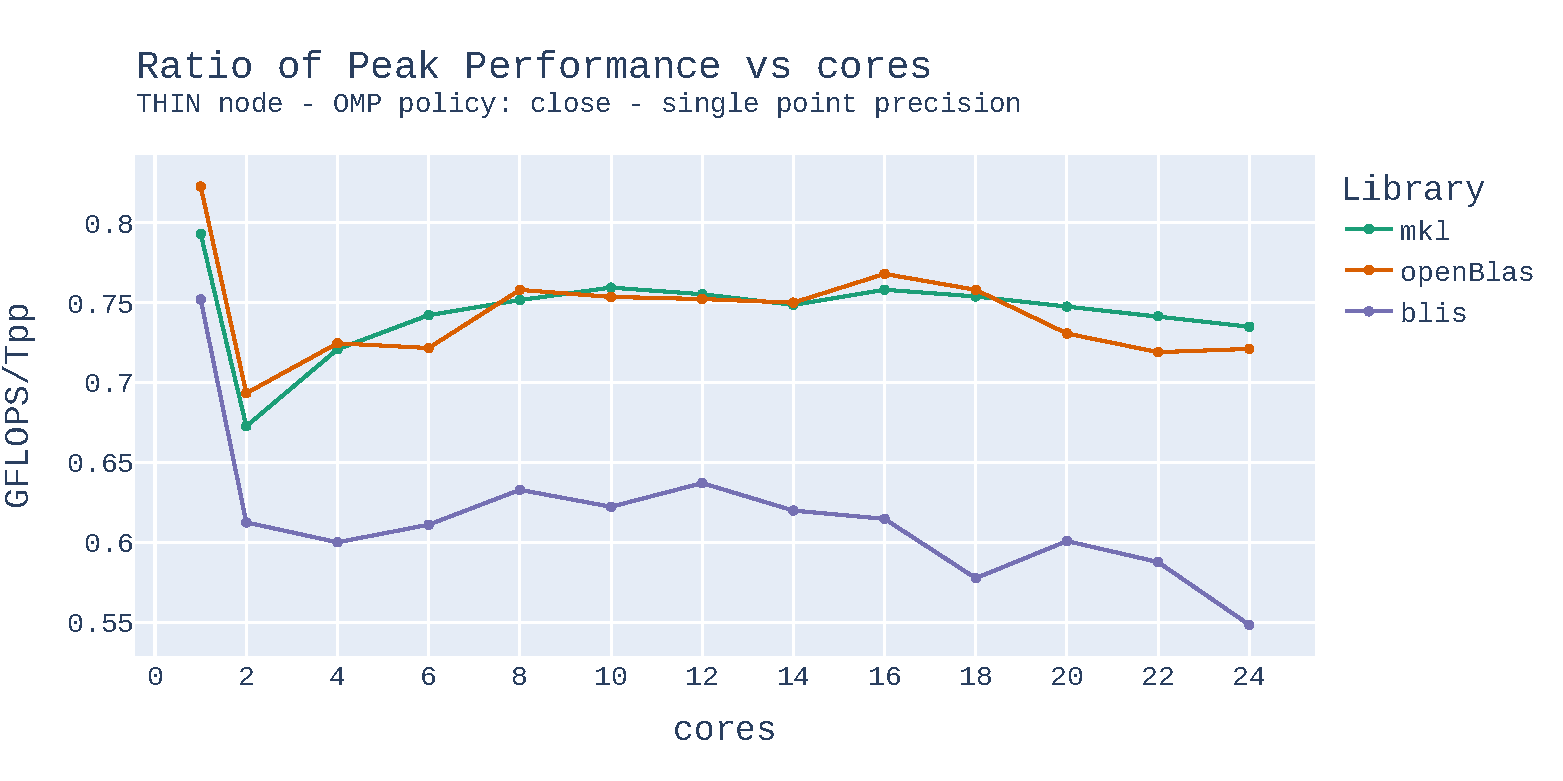
\includegraphics[width=10cm, height=6cm]{./images/fixed_size_thin_float_gflops_close_ratio.pdf}
\caption{\label{fig:fixed_size_thin_float_close} Results of SP matrix-matrix multiplication 
    as the number of cores increase, using close policy.}
\end{figure}

\texttt{MKL} and \texttt{OpenBLAS} are able to maintain $\sim 75\%$
of $T_{pp}$ from $6$ cores and onwards. On the other hand, \texttt{BLIS}
is able to achieve $\sim 60\%$ of $T_{pp}$, although with a lot of cores, 
this figure decreases to $55\%$. These numbers are consistent with the results 
that we obtained previously. 

Interestingly, we notice that with $2$ cores, there is a significant performance 
drop. This is most likely explained by the fact that both cores are mapped to the 
same socket and must share resources, such as the higher level caches.

In conclusion, once again, we notice that the best performing library is \texttt{MKL}
which is Intel based, closely followed by \texttt{OpenBLAS}.

\begin{figure}[h!]
% \centering
\hspace*{-2.5cm}
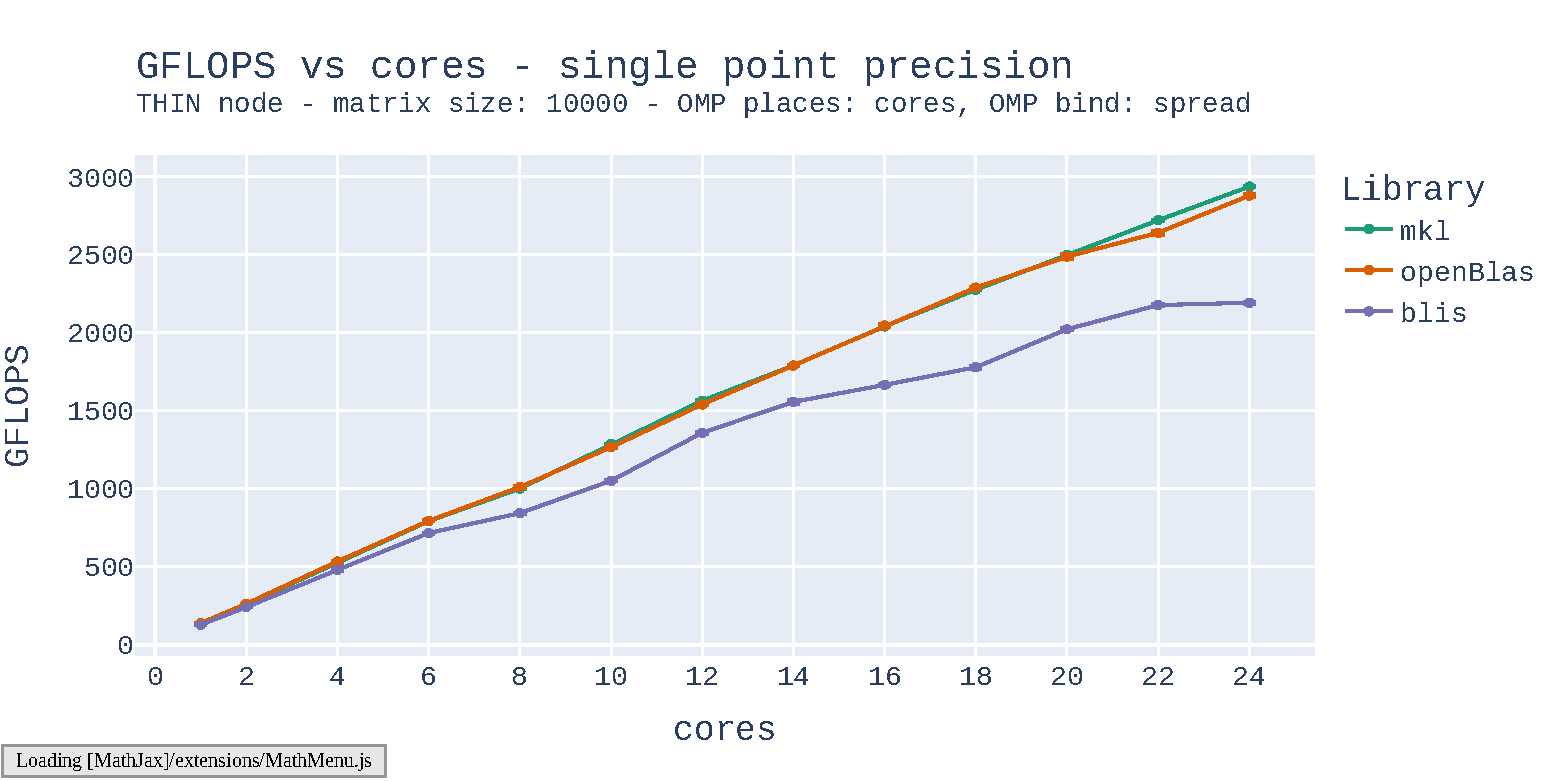
\includegraphics[width=10cm, height=6cm]{./images/fixed_size_thin_float_gflops_spread.pdf}
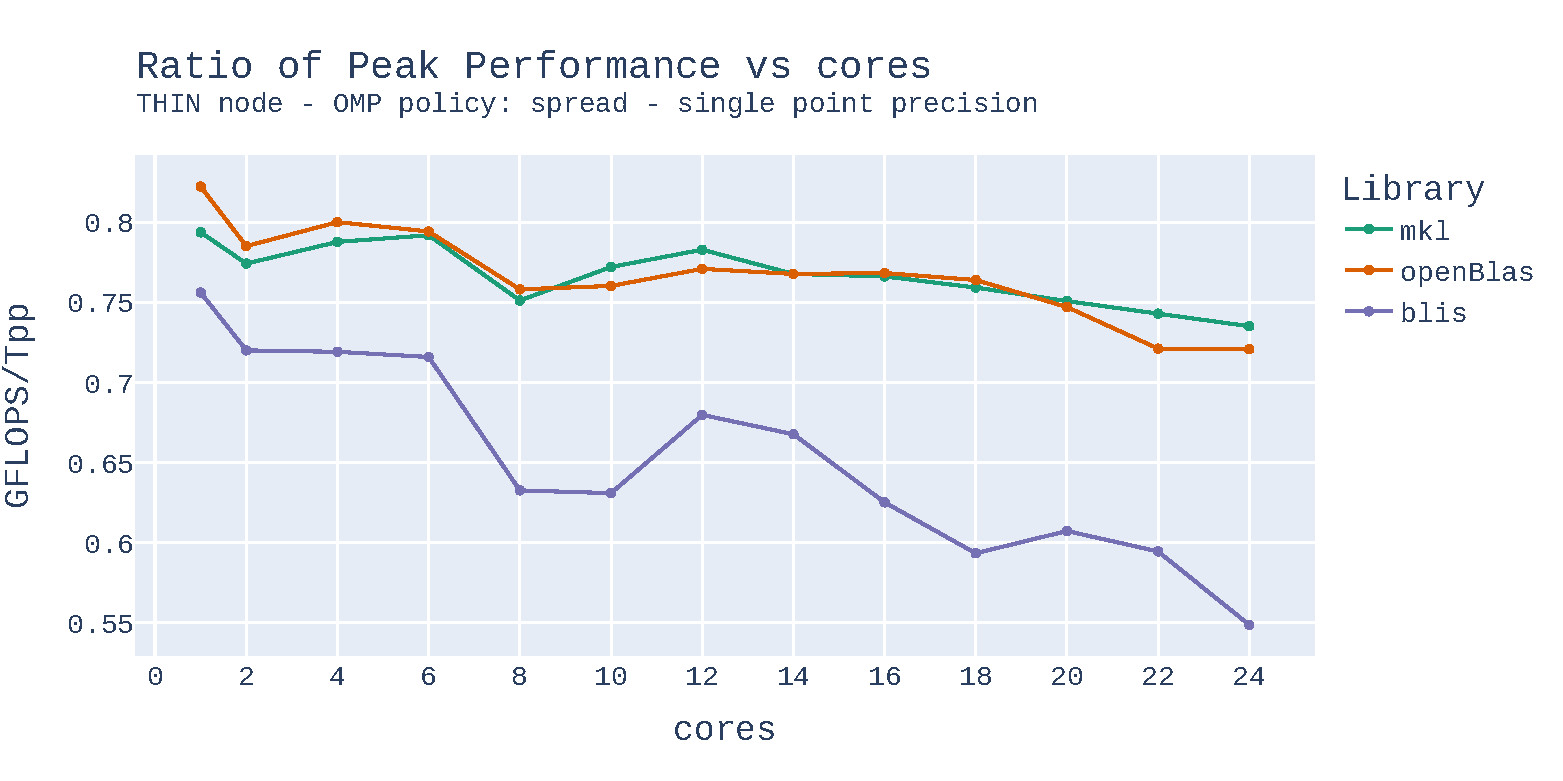
\includegraphics[width=10cm, height=6cm]{./images/fixed_size_thin_float_gflops_spread_ratio.pdf}
\caption{\label{fig:fixed_size_thin_float_spread} Results of SP matrix-matrix multiplication 
as the number of cores increase, using spread policy.}
\end{figure}

Using a spread policy, we obtain very similar results to the case where we use 
a close policy. The main difference is that we don't have the same performance 
drop at 2 cores. This is most likely due to the fact that with a spread policy, 
each core is mapped to its own socket and there is no contention for resources. 

In fact, we notice that on average, the performance is slightly better than the 
close policy counterpart, and this is probably due to better resource sharing 
from the beginning.

This highlights the importance of using the correct mapping policy to obtain better 
performance.

Now we briefly analyze the results obtained for double precision.
\begin{figure}[h!]
% \centering
\hspace*{-2.5cm}
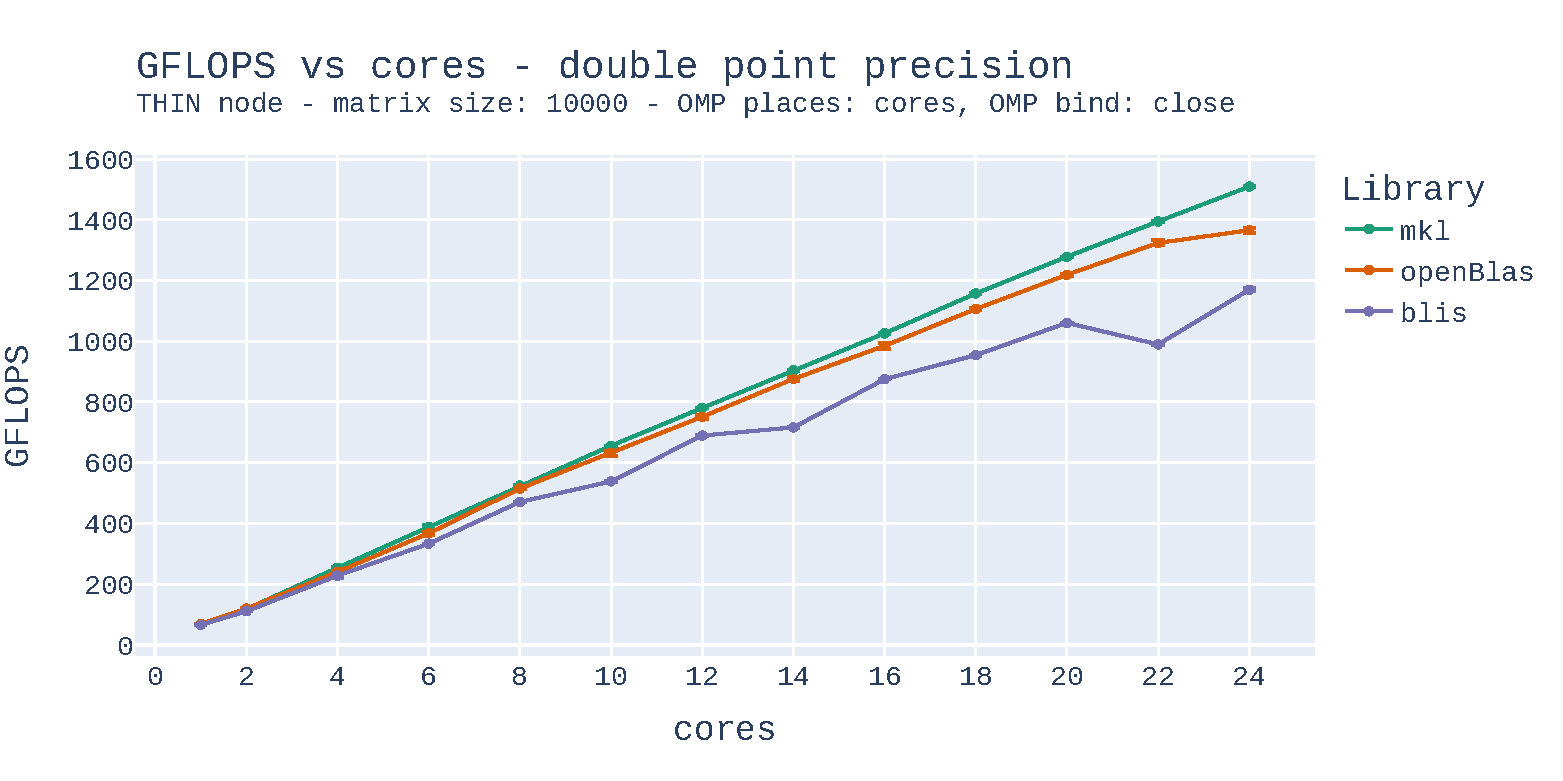
\includegraphics[width=10cm, height=6cm]{./images/fixed_size_thin_double_gflops_close.pdf}
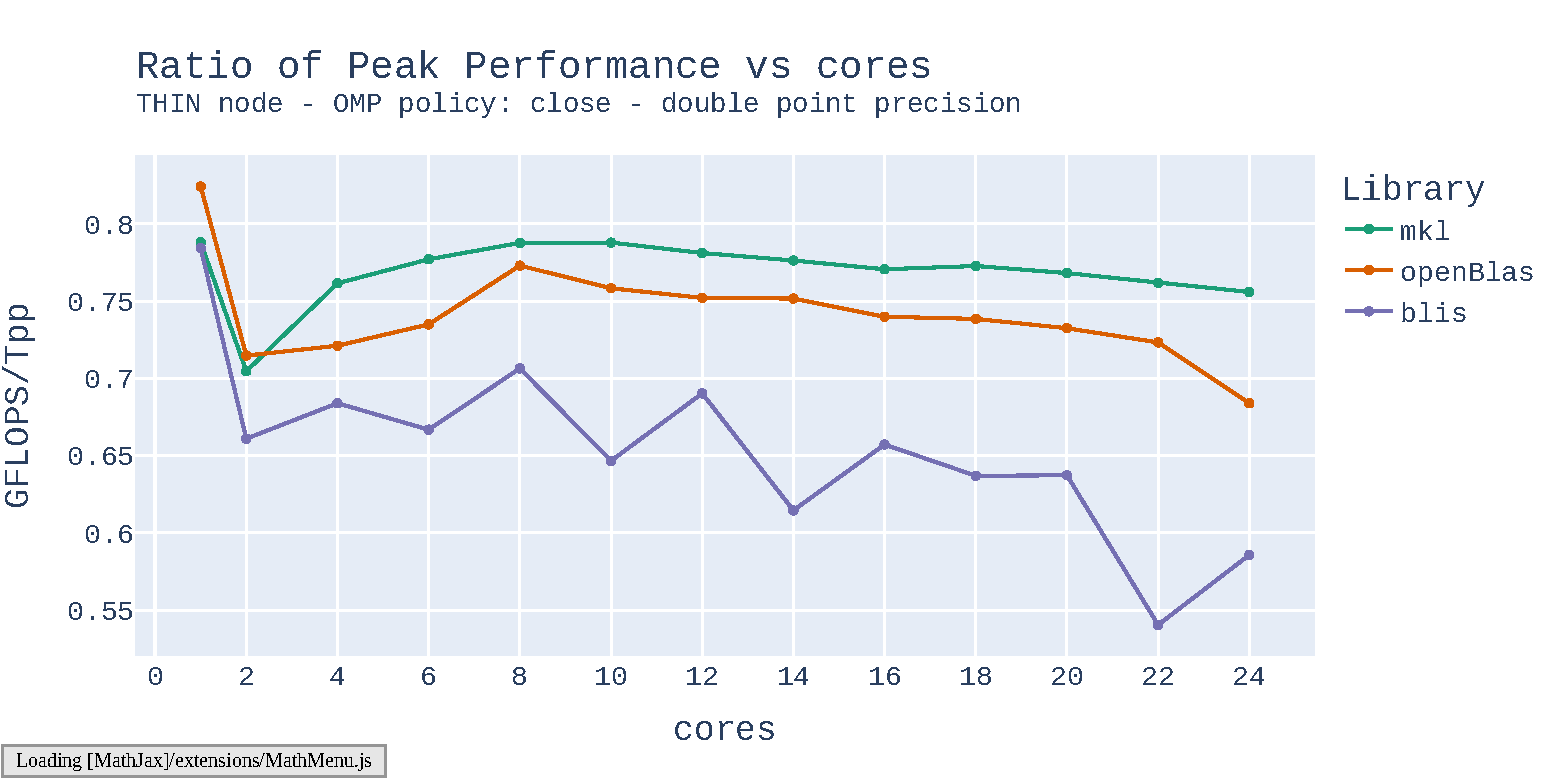
\includegraphics[width=10cm, height=6cm]{./images/fixed_size_thin_double_gflops_close_ratio.pdf}
\caption{\label{fig:fixed_size_thin_double_close} Results of DP matrix-matrix multiplication 
    as the number of cores increase, using close policy.}
\end{figure}

\begin{figure}[h!]
% \centering
\hspace*{-2.5cm}
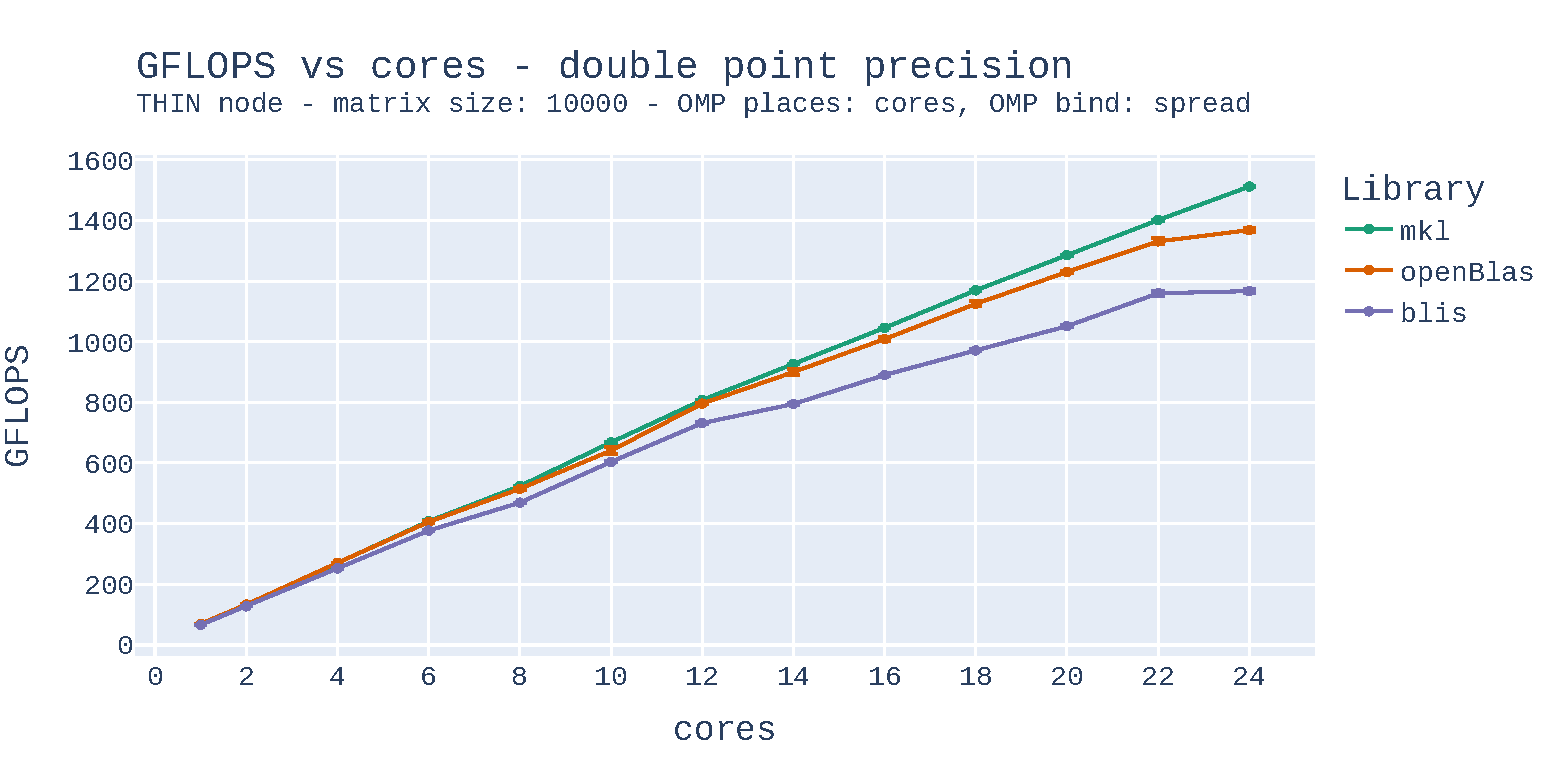
\includegraphics[width=10cm, height=6cm]{./images/fixed_size_thin_double_gflops_spread.pdf}
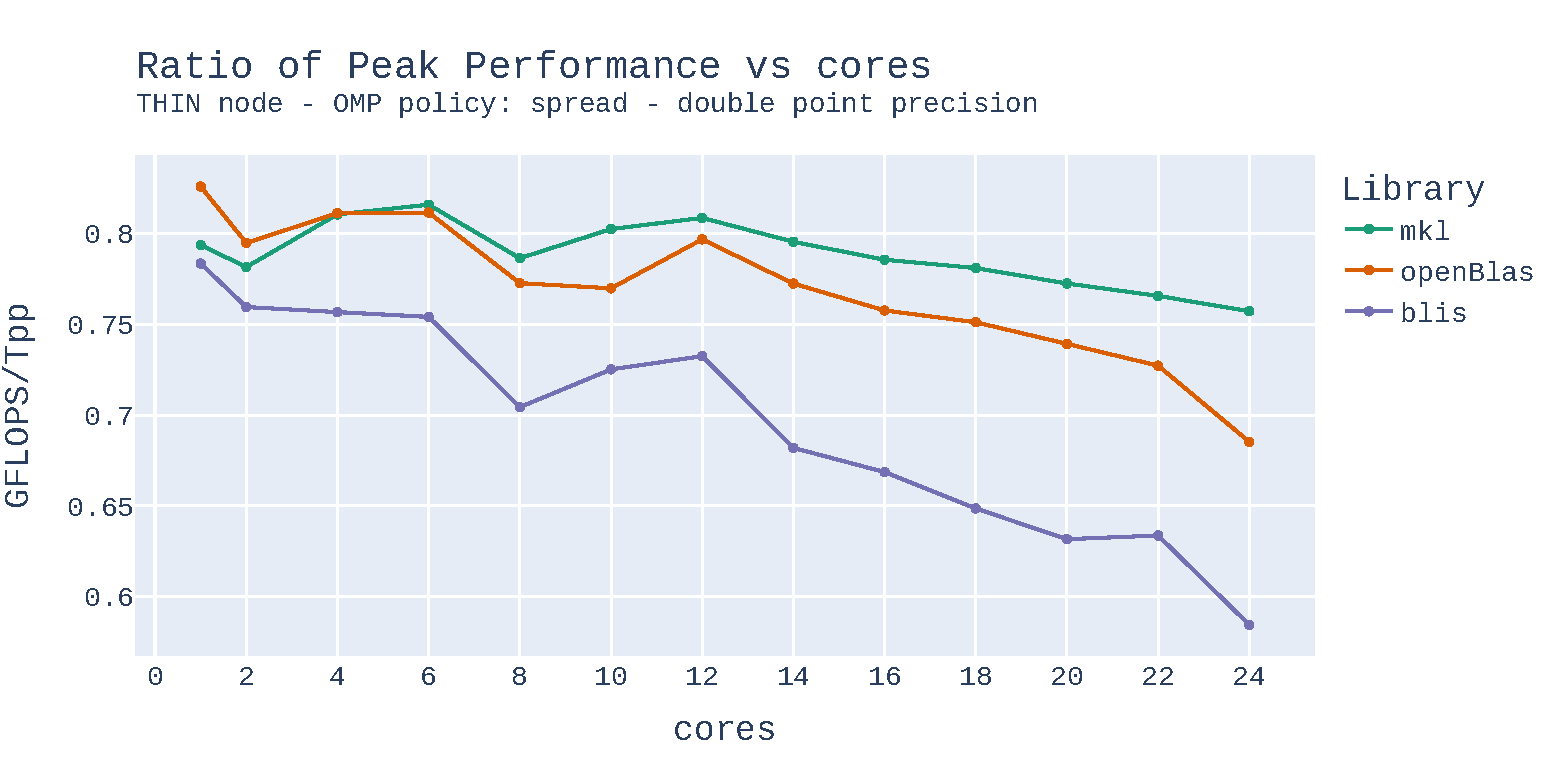
\includegraphics[width=10cm, height=6cm]{./images/fixed_size_thin_double_gflops_spread_ratio.pdf}
\caption{\label{fig:fixed_size_thin_double_spread} Results of DP matrix-matrix multiplication 
as the number of cores increase, using spread policy.}
\end{figure}

The analysis and discussion is very similar to the case of single point precision. 
As usual, \texttt{MKL}, which is Intel based, performs the best, closely followed 
by \texttt{OpenBLAS}, and finally, \texttt{BLIS} performs the worst. 

The percentage of $T_{pp}$ achieved is rather similar, with \texttt{OpenBLAS} performing 
slightly worse.

\subsubsection{EPYC Nodes}

We discuss the situation on EPYC nodes. Considering the results of the first part 
of the exercise, we expect that \texttt{MKL} won't be the dominating library to 
perform matrix-matrix multiplication since we are using an AMD architecture.

\begin{figure}[h]
% \centering
\hspace*{-2.5cm}
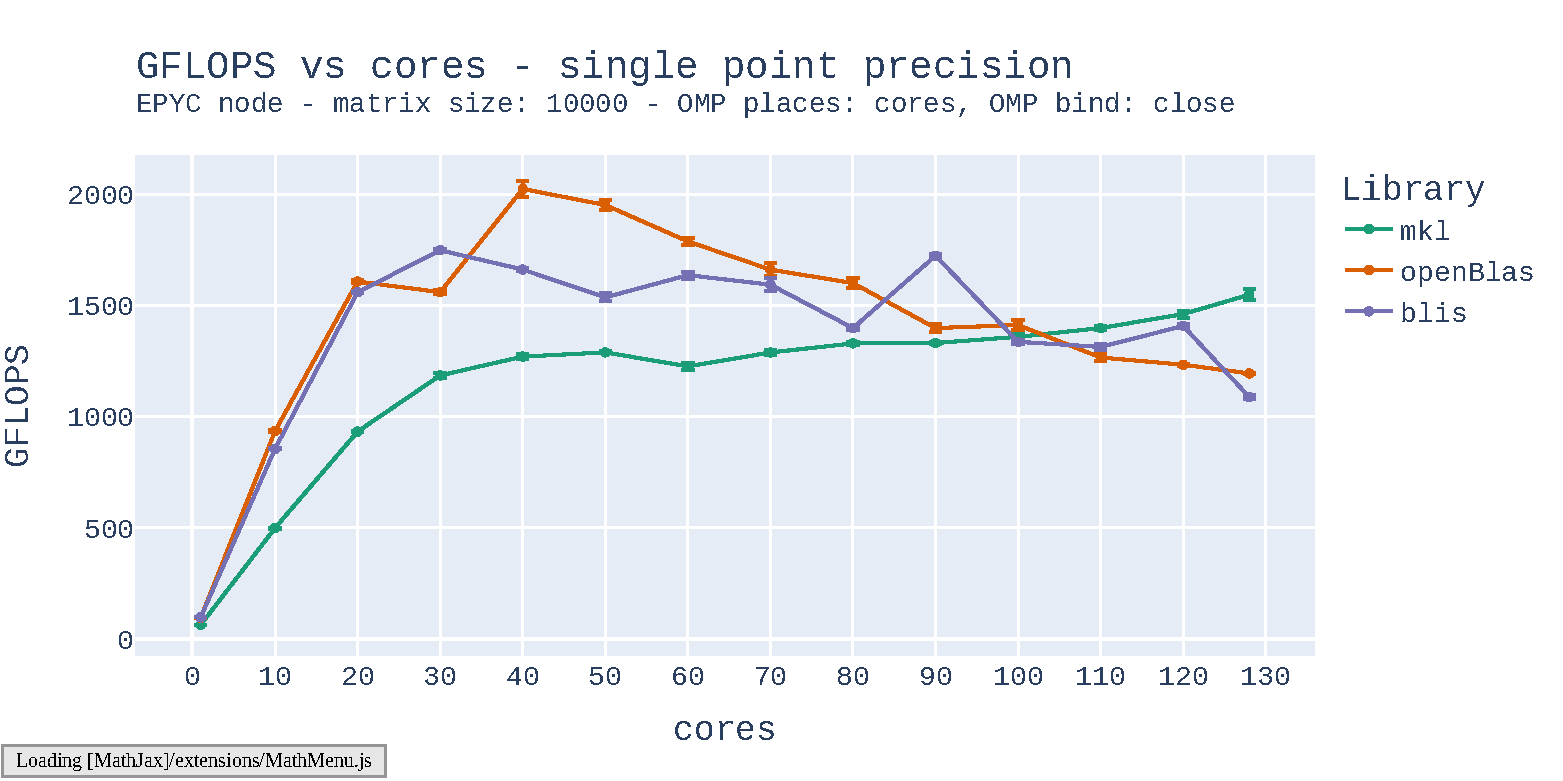
\includegraphics[width=10cm, height=6cm]{./images/fixed_size_epyc_float_gflops_close.pdf}
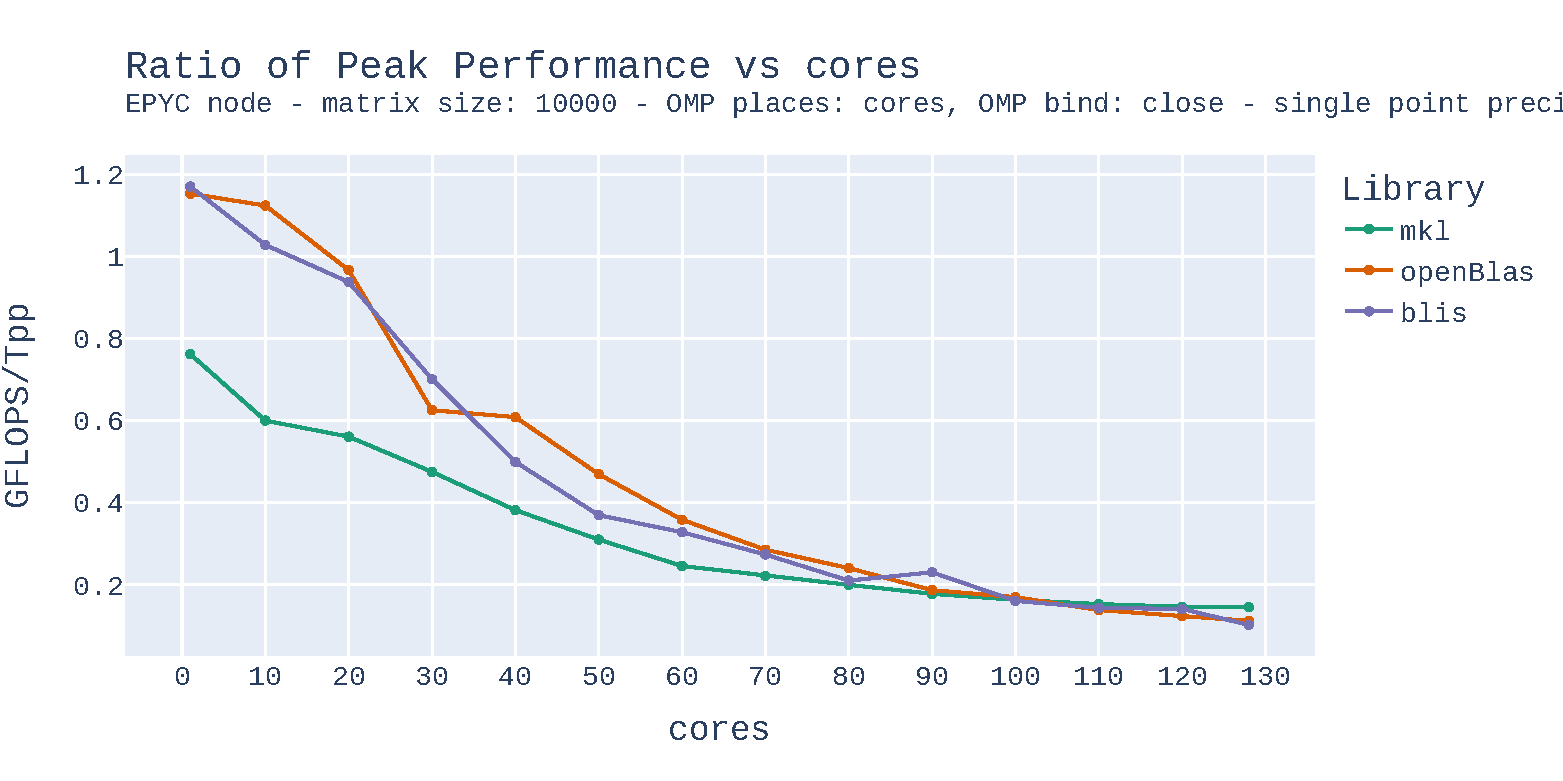
\includegraphics[width=10cm, height=6cm]{./images/fixed_size_epyc_float_gflops_close_ratio.pdf}
\caption{\label{fig:fixed_size_epyc_float} }
\end{figure}

\begin{figure}[h]
% \centering
\hspace*{-2.5cm}
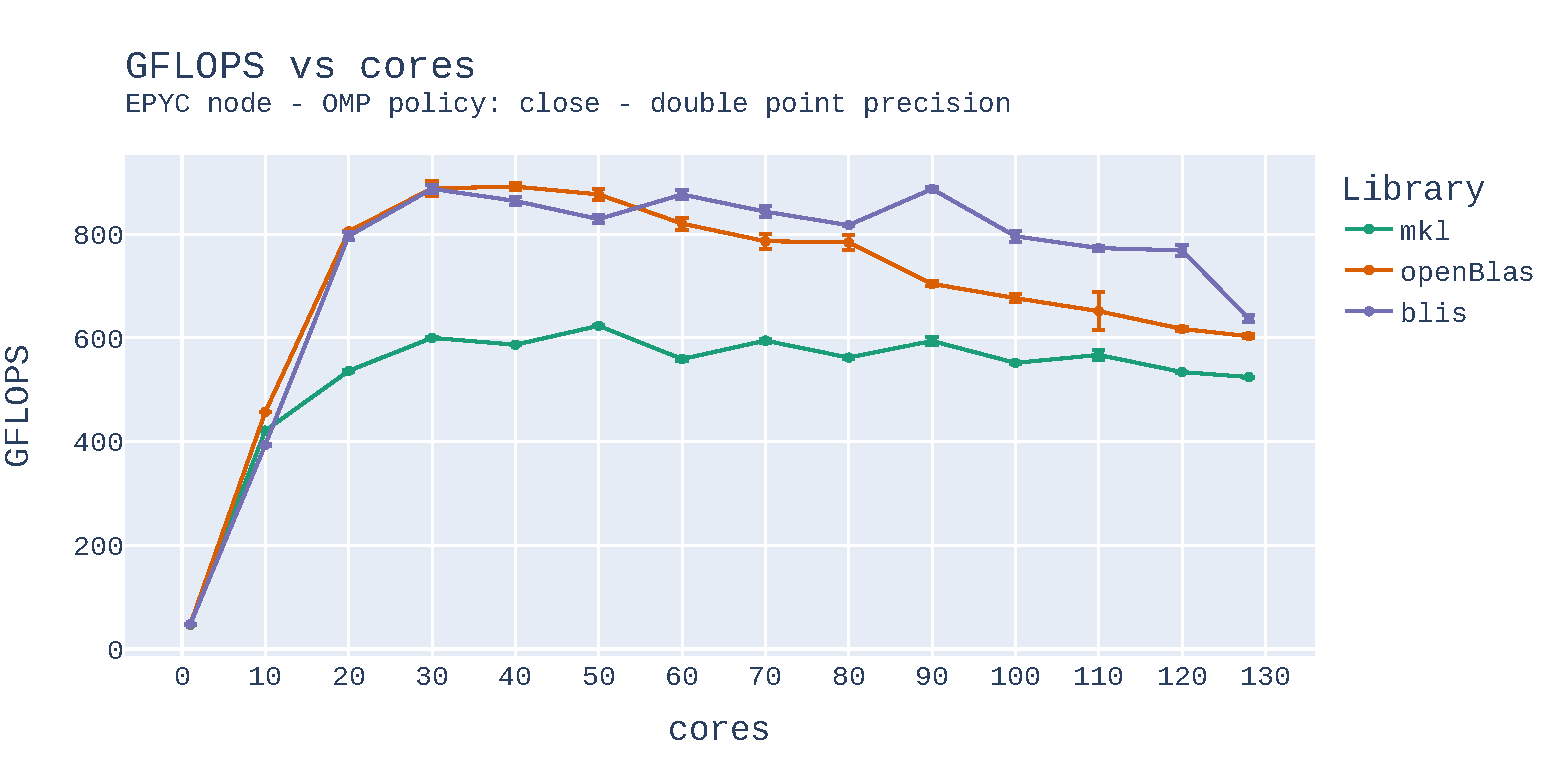
\includegraphics[width=10cm, height=6cm]{./images/fixed_size_epyc_double_gflops_close.pdf}
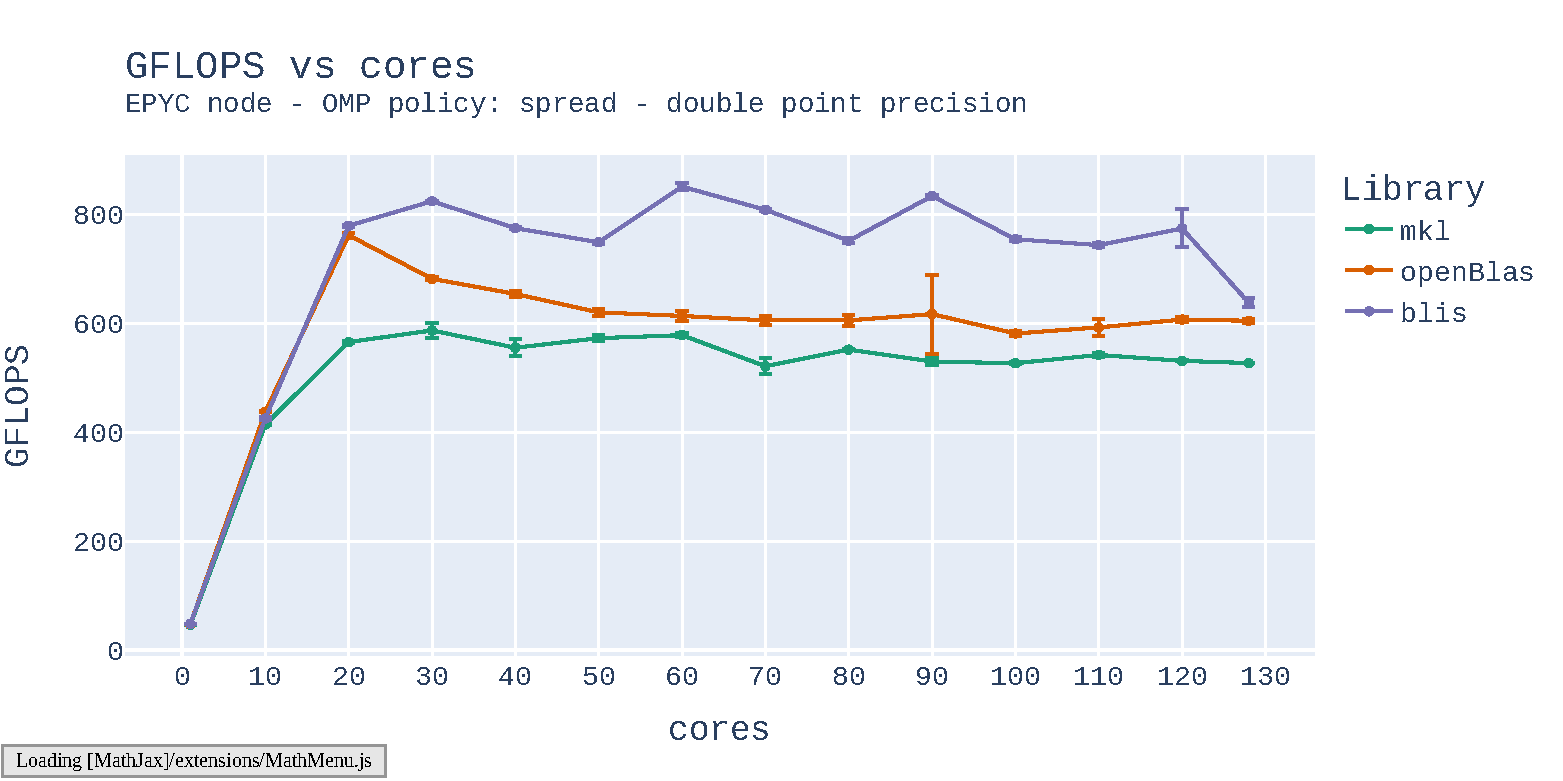
\includegraphics[width=10cm, height=6cm]{./images/fixed_size_epyc_double_gflops_spread.pdf}
\caption{\label{fig:fixed_size_epyc_double} }
\end{figure}

\section{Conclusion}


\chapter{Conway's Game of Life}


\section{Introduction}

This exercise is devoted to implementing a scalable version of Conway's Game of 
life\cite{conway}. The game consists of a $k\times k$ grid, where each cell can 
be "alive" or "dead".

The grid evolves over time by looking at a cell's $\mathcal{C}$ eight nearest 
neighbors and observing the following simple rules: 

\begin{itemize}
    \item A dead cell with exactly three live neighbors comes to live (\textit{birth}).
    \item A live cell with two or three neighbors stays alive (\textit{survival}).
    \item A dead or live cell less than two or more than three neighbors dies 
        or stays dead by under or overpolulation, respectively (\textit{death}).
\end{itemize}

These seemingly simple rules give rise to many interesting behaviors and patterns.

Depending on how we update the cells, there exist two methods to evolve the 
grid: \texttt{static} and \texttt{ordered}. In \texttt{static} evolution, we 
freeze the state of the grid $\mathcal{G}_t$ at time step $t$, and compute 
$\mathcal{G}_{t+1}$ separately, while looking at $\mathcal{G}_t$.

On the other hand, in \texttt{ordered} evolution, we start from a specific cell, 
usually in position $(0,0)$ (top left), and update the elements in\-place. 
In this scenario, the state of each cell depends on the evolution of all the 
cells before it. 

Our implementation must satisfy the following requirements: 

\begin{enumerate}
    \item Randomly initialize a square grid ("playground") of size $k \times k$ 
        with $k \geq 100$ and save it as a binary PGM file.
    \item Load a binary PGM file and evolve for $n$ steps.
    \item Save a snapshot during the course of evolution with frequency $s$ ($s=0$ 
        means save at the end). 
    \item Support both \texttt{static} and \texttt{ordered} evolution.
\end{enumerate}

Lastly, it must use both MPI\cite{mpi} and OpenMP\cite{omp} to paralellize 
the computations and be able to process grids of considerably high dimensions. 

\section{Methodology}

Since programs in MPI need to be rewritten completely from their serial 
counterparts, we must begin to conceptualize the problem in an encapsulated 
manner from the start.

At a high abstract level, we must make two important choices: 

\begin{enumerate}
    \item How we will decompose the problem. 
    \item How we will perform the IO (this has important consequences on the 
        organizational paradigm we will use).
\end{enumerate}

We briefly discuss both of these topics more in depth in the following subsections.

\subsection{Problem decomposition}

To exploit paralellism, we must first identify the concurrency in our 
application and then apply some form of decomposition. The two most important 
types of decomposition are \texttt{domain} and \texttt{functional} decomposition. 

In domain decomposition, multiple workers are performing the same set of 
instructions on different portions of data (SIMD). In functional 
decomposition, workers are performing different instructions on possibly 
different data (MIMD). 
 
In the case of static evolution, each cell can be updated independently from each 
other, as long as we have acccess to its neighbors. Therefore, one immediately 
obviously form of paralellism is for each MPI process to update their "part" 
of the whole grid. 

For this, we need to decide how to split the grid since we can do both a 1D or 
2D decomposition of our grid. It is known that a 2D decomposition is more 
efficient as it can exploit more bandwidth (more workers will send shorter messages 
at the same time). However, it is more complicated both from an implementation 
point of view, as well as it is worse for memory access. 

Let's talk briefly about this second aspect. Although we will talk about our 
grid as a 2D array, internally, for efficiency, it will be represented as a 1D 
array. Therefore, each process will work on a strip of continuous data as 
shown in the figure below. 

\begin{figure}[h]
\centering
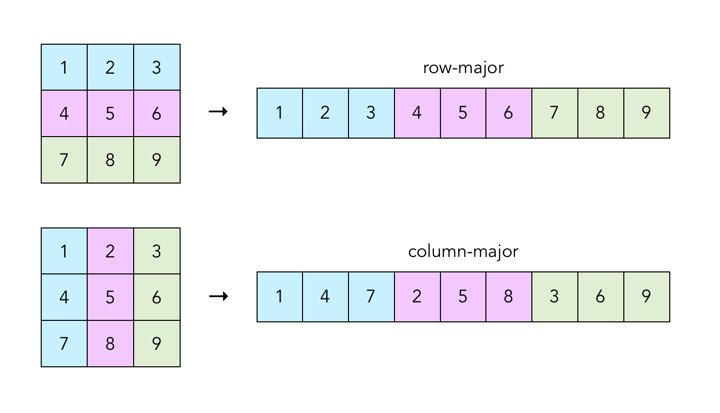
\includegraphics[width=10cm, height=5cm]{./other_images/arraydecomposition.jpg}
\caption{\label{fig:decomposition}.}
\end{figure}


Fas one long array, in a 1D split, each process will need to work on a continuous


"strip" of this memory. 



\section{Implementation}

\section{Results and Discussion}

\section{Conclusions}

\subsection{How to add Tables}

% Use the table and tabular environments for basic tables --- see Table~\ref{tab:widgets}, for example. For more information, please see this help article on \href{https://www.overleaf.com/learn/latex/tables}{tables}. 
%
% \begin{table}
% \centering
% \begin{tabular}{l|r}
% Item & Quantity \\\hline
% Widgets & 42 \\
% Gadgets & 13
% \end{tabular}
% \caption{\label{tab:widgets}An example table.}
% \end{table}
%
% \subsection{How to add Comments and Track Changes}
%
% Comments can be added to your project by highlighting some text and clicking ``Add comment'' in the top right of the editor pane. To view existing comments, click on the Review menu in the toolbar above. To reply to a comment, click on the Reply button in the lower right corner of the comment. You can close the Review pane by clicking its name on the toolbar when you're done reviewing for the time being.
%
% Track changes are available on all our \href{https://www.overleaf.com/user/subscription/plans}{premium plans}, and can be toggled on or off using the option at the top of the Review pane. Track changes allow you to keep track of every change made to the document, along with the person making the change. 
%
% \subsection{How to add Lists}
%
% You can make lists with automatic numbering \dots
%
% \begin{enumerate}
% \item Like this,
% \item and like this.
% \end{enumerate}
% \dots or bullet points \dots
% \begin{itemize}
% \item Like this,
% \item and like this.
% \end{itemize}
%
% \subsection{How to write Mathematics}
%
% \LaTeX{} is great at typesetting mathematics. Let $X_1, X_2, \ldots, X_n$ be a sequence of independent and identically distributed random variables with $\text{E}[X_i] = \mu$ and $\text{Var}[X_i] = \sigma^2 < \infty$, and let
% \[S_n = \frac{X_1 + X_2 + \cdots + X_n}{n}
%       = \frac{1}{n}\sum_{i}^{n} X_i\]
% denote their mean. Then as $n$ approaches infinity, the random variables $\sqrt{n}(S_n - \mu)$ converge in distribution to a normal $\mathcal{N}(0, \sigma^2)$.
%
%
% \subsection{How to change the margins and paper size}
%
% Usually the template you're using will have the page margins and paper size set correctly for that use-case. For example, if you're using a journal article template provided by the journal publisher, that template will be formatted according to their requirements. In these cases, it's best not to alter the margins directly.
%
% If however you're using a more general template, such as this one, and would like to alter the margins, a common way to do so is via the geometry package. You can find the geometry package loaded in the preamble at the top of this example file, and if you'd like to learn more about how to adjust the settings, please visit this help article on \href{https://www.overleaf.com/learn/latex/page_size_and_margins}{page size and margins}.
%
% \subsection{How to change the document language and spell check settings}
%
% Overleaf supports many different languages, including multiple different languages within one document. 
%
% To configure the document language, simply edit the option provided to the babel package in the preamble at the top of this example project. To learn more about the different options, please visit this help article on \href{https://www.overleaf.com/learn/latex/International_language_support}{international language support}.
%
% To change the spell check language, simply open the Overleaf menu at the top left of the editor window, scroll down to the spell check setting, and adjust accordingly.
%
% \subsection{How to add Citations and a References List}
%
% You can simply upload a \verb|.bib| file containing your BibTeX entries, created with a tool such as JabRef. You can then cite entries from it, like this: \cite{greenwade93}. Just remember to specify a bibliography style, as well as the filename of the \verb|.bib|. You can find a \href{https://www.overleaf.com/help/97-how-to-include-a-bibliography-using-bibtex}{video tutorial here} to learn more about BibTeX.
%
% If you have an \href{https://www.overleaf.com/user/subscription/plans}{upgraded account}, you can also import your Mendeley or Zotero library directly as a \verb|.bib| file, via the upload menu in the file-tree.
%
% \subsection{Good luck!}
%
% We hope you find Overleaf useful, and do take a look at our \href{https://www.overleaf.com/learn}{help library} for more tutorials and user guides! Please also let us know if you have any feedback using the Contact Us link at the bottom of the Overleaf menu --- or use the contact form at \url{https://www.overleaf.com/contact}.

\printbibliography

\end{document}
